\documentclass[journal,twoside]{IEEEtran}

\usepackage{amsmath,amssymb}
\usepackage{booktabs}
\usepackage{graphicx}
\usepackage{multirow}
\usepackage{xcolor}
\usepackage{cite}
\usepackage[hidelinks]{hyperref}

\newcommand{\method}{CTF-GS}
\newcommand{\project}{RADIO-GS}
\newcommand{\radio}{C-RADIOv4-H}

\title{\method{}: Compact Foundation-Feature Gaussian Memory for Open-Vocabulary 3D Scene Understanding}

\author{Anonymous Authors%
\thanks{Manuscript prepared for IEEE Transactions on Pattern Analysis and Machine Intelligence.}}
\markboth{IEEE Transactions on Pattern Analysis and Machine Intelligence,~Vol.~XX, No.~XX, 2026}%
{\method{}: Compact Foundation-Feature Gaussian Memory for Open-Vocabulary 3D Scene Understanding}

\begin{document}
\maketitle

\begin{abstract}
Dense vision foundation models provide strong 2D features, but deployed 3D
scenes still lack a compact scene memory that can carry those features across
novel views, Gaussian primitives, and point-query protocols. We present
\method{}, a compact foundation-feature Gaussian memory for 3D scenes. Rather
than storing raw 1280-D RADIO features on every Gaussian or training a
scene-specific classifier, \method{} stores low-dimensional per-Gaussian latent
codes, augments them with spatial context and reliability cues, and reconstructs
RADIO-compatible scene features on demand. Training combines dense rendered
RADIO reconstruction with sparse Multiview Primitive Registration, which
compresses registered multiview semantic evidence back into the same compact
Gaussian memory. The resulting representation supports rendered 2D querying,
direct primitive selection, and direct point querying without deploying a
multiview feature cache.

We evaluate \method{} under three protocols. On LERF-OVS rendered-view
open-vocabulary query, \method{} reaches 64.98 mIoU and 82.68 Acc. Under the
same LERF-OVS direct 3D query-select-render protocol, compact primitive scoring
with support calibration reaches 54.36 mIoU and 80.84 Acc without
reading a multiview-registration cache or invoking an official RGB SAM decoder
at inference. On the VALA-aligned ScanNet-8 direct point-query protocol, the
compact field reaches 36.55, 42.78, and 57.85 mIoU on the 19-, 15-, and
10-class splits. Same-evaluator frame-wise foundation-feature comparisons
and component ablations show that multiview reconstruction, sparse primitive
anchoring, and support-calibrated 3D selection drive the gains. Small
fragmented objects remain the primary failure mode.
\end{abstract}

\begin{IEEEkeywords}
Open-vocabulary 3D scene understanding, 3D Gaussian Splatting, vision foundation models, feature distillation, scene representation.
\end{IEEEkeywords}

\section{Introduction}

Vision foundation models expose dense features that are useful for recognition,
localization, segmentation, and geometric reasoning. However, most 3D scene
representations still optimize either RGB appearance or task-specific labels. In
open-vocabulary 3D understanding, this creates a gap: the strongest 2D feature
extractors are available at training images, but a deployed 3D scene must answer
queries from novel views, select objects directly in 3D, and transfer to new
point-query protocols without storing a dense RADIO feature on every
primitive.

\method{} targets this gap by reconstructing foundation-model features inside a
3D Gaussian scene. Our goal is not to train a new per-scene language classifier.
Instead, we ask whether one compact scene memory can support multiple query
modes: dense novel-view feature maps for rendered open-vocabulary localization,
direct primitive scores for 3D object selection, and point-level features for
semantic querying. This
feature-reconstruction framing differs from
methods that attach only a final language code to a radiance field or optimize a
single downstream score.

The technical challenge is that RADIO features are high-dimensional, dense, and
expensive to store directly on every Gaussian. We therefore learn a compact
Contextual Gaussian Feature Field, reconstruct foundation-compatible features
through a Foundation-Space Reconstruction module, and calibrate them in view
space before comparison to frozen RADIO targets. We also use Frozen-Head
Geometry Consistency as a geometry-aware regularizer: a frozen downstream head
guides the feature field without turning the model into a task-specific
predictor.

We evaluate this formulation with a protocol boundary that mirrors recent
open-vocabulary Gaussian-field papers. LERF-OVS rendered-view grounding tests
whether the field can produce dense novel-view features; LERF direct 3D object
selection tests whether text queries can select Gaussian primitives before any
rendered-mask evaluation; and VALA-aligned ScanNet-8 direct point querying
tests whether the same compact representation remains usable outside the LERF
object-query setting. Baseline comparisons in the main LERF and ScanNet tables
follow the same reproduced protocols as \method{}, while historical provenance
audits are kept in the appendix.

\paragraph{Contributions.}
We make three contributions:
\begin{itemize}
  \item We introduce a compact reconstructive RADIO Gaussian feature field:
  low-dimensional per-Gaussian latent codes, spatial context, reliability
  modeling, and global decoders replace explicit high-dimensional feature
  storage while preserving foundation-feature usability.
  \item We combine dense rendered RADIO reconstruction with sparse
  Multiview Primitive Registration and support calibration, so the same compact
  memory supports rendered 2D querying, direct 3D primitive selection, and
  ScanNet point-level querying without a deployed multiview feature cache.
  \item We provide a protocol-separated evaluation covering LERF-OVS 2D and
  3D open-vocabulary query, VALA-aligned ScanNet point query, frame-wise
  RADIO versus reconstructed scene features, storage/latency, qualitative
  analysis, and component ablations.
\end{itemize}

\begin{figure*}[t]
\centering
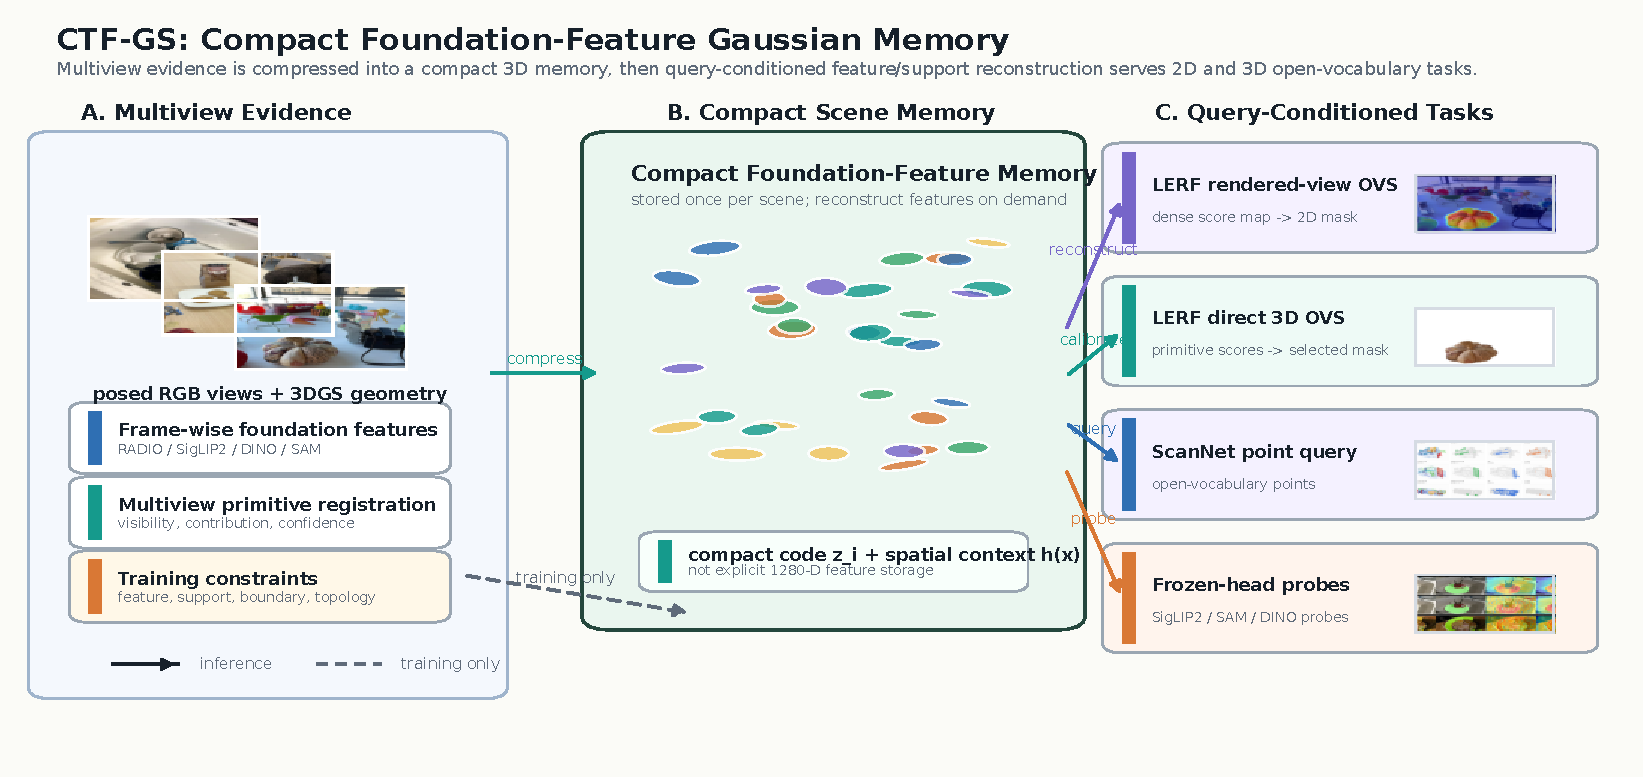
\includegraphics[width=\linewidth]{figures/figure1_overall_framework.pdf}
\caption{\method{} framework. A pretrained 3DGS scene supplies geometry, while
frozen RADIO supplies the dense foundation feature to be reconstructed. The
method stores compact per-Gaussian latent codes with spatial context and
quality/visibility cues, then reconstructs RADIO-compatible scene features by
global decoders. SigLIP2, DINOv3, and SAM3 adaptor spaces are used as
frozen-head constraints or probes of the reconstructed RADIO feature, not as
separate raw feature memories. Multiview Primitive Registration compresses
registered semantic evidence into the same compact memory during training.
At inference, the memory supports rendered 2D query, direct Gaussian selection,
and point-level query without a multiview-registration feature cache or official
RGB SAM decoder.}
\label{fig:framework}
\end{figure*}

\section{Related Work}

\paragraph{Language fields and open-vocabulary 3D understanding.}
LERF embeds language-aligned features in neural radiance fields and enables
open-vocabulary querying in 3D scenes~\cite{kerr2023lerf}. LangSplat and
Language Embedded 3D Gaussians adapt this direction to Gaussian scene
representations~\cite{qin2024langsplat,shi2024legaussians}. OpenGaussian
formalizes a stronger primitive-level protocol in which text selects 3D
Gaussians that are then rendered only for mask
evaluation~\cite{wu2024opengaussian}. Recent methods push this direction
further: Dr. Splat registers language-aligned features directly to dominant
Gaussians along pixel rays~\cite{kim2025drsplat}, while InstanceGaussian and
OpenSplat3D move toward instance-level Gaussian grouping
and open-vocabulary instance segmentation~\cite{li2025instancegaussian,piekenbrinck2025opensplat3d}.
OpenInsGaussian further studies context-aware cross-view fusion for instance
Gaussian segmentation~\cite{huang2025openinsgaussian}, while very recent
Ilov3Splat uses view-consistent feature fields and two-stage 3D clustering for
instance-level open-vocabulary querying~\cite{nguyen2026ilov3splat}.
SuperGSeg clusters Gaussians into structured super-primitives for hierarchical
understanding~\cite{liang2026supergseg}. These methods demonstrate that
Gaussian scenes can carry language-aligned evidence, but they mostly store or
aggregate final semantic embeddings. They do not directly answer whether a
3DGS scene can be a compact reconstructive memory for a high-dimensional
foundation feature while retaining rendered-view, primitive-level, point-level,
and frozen-head downstream usability. \method{} targets this gap by
reconstructing RADIO-compatible features from low-dimensional Gaussian codes and
compressing registered multiview evidence back into the same primitive-level
memory.

\paragraph{Gaussian scene representations.}
3D Gaussian Splatting provides an explicit and efficient scene representation
for radiance-field rendering~\cite{kerbl2023gaussians}. \method{} keeps this
geometry backbone and learns a feature field on top of it, separating geometric
visibility from foundation-feature reconstruction.

\paragraph{Agglomerative vision foundation models.}
RADIO-style models distill multiple visual capabilities into a single dense
vision backbone~\cite{ranzinger2024radio,nvidia2026cradiov4}. \method{} uses
\radio{} as a frozen feature source and studies whether its dense features can be
reconstructed from 3D scenes at novel views.

\paragraph{Foundation-model regularization in 3DGS.}
FMGS embeds 2D foundation-model features into Gaussian scenes and uses DINO-style
spatial structure to improve feature consistency~\cite{liu2024fmgs}. SAM-based
Gaussian methods such as SAGA distill 2D segmentation priors into 3D Gaussian
features for promptable object segmentation~\cite{cen2023saga}. Our adaptor
regularizers follow the same principle, but use the official \radio{} adaptor
heads so that the reconstructed feature remains a single RADIO-compatible
representation at inference time.

\section{Method}

\begin{figure*}[t]
\centering
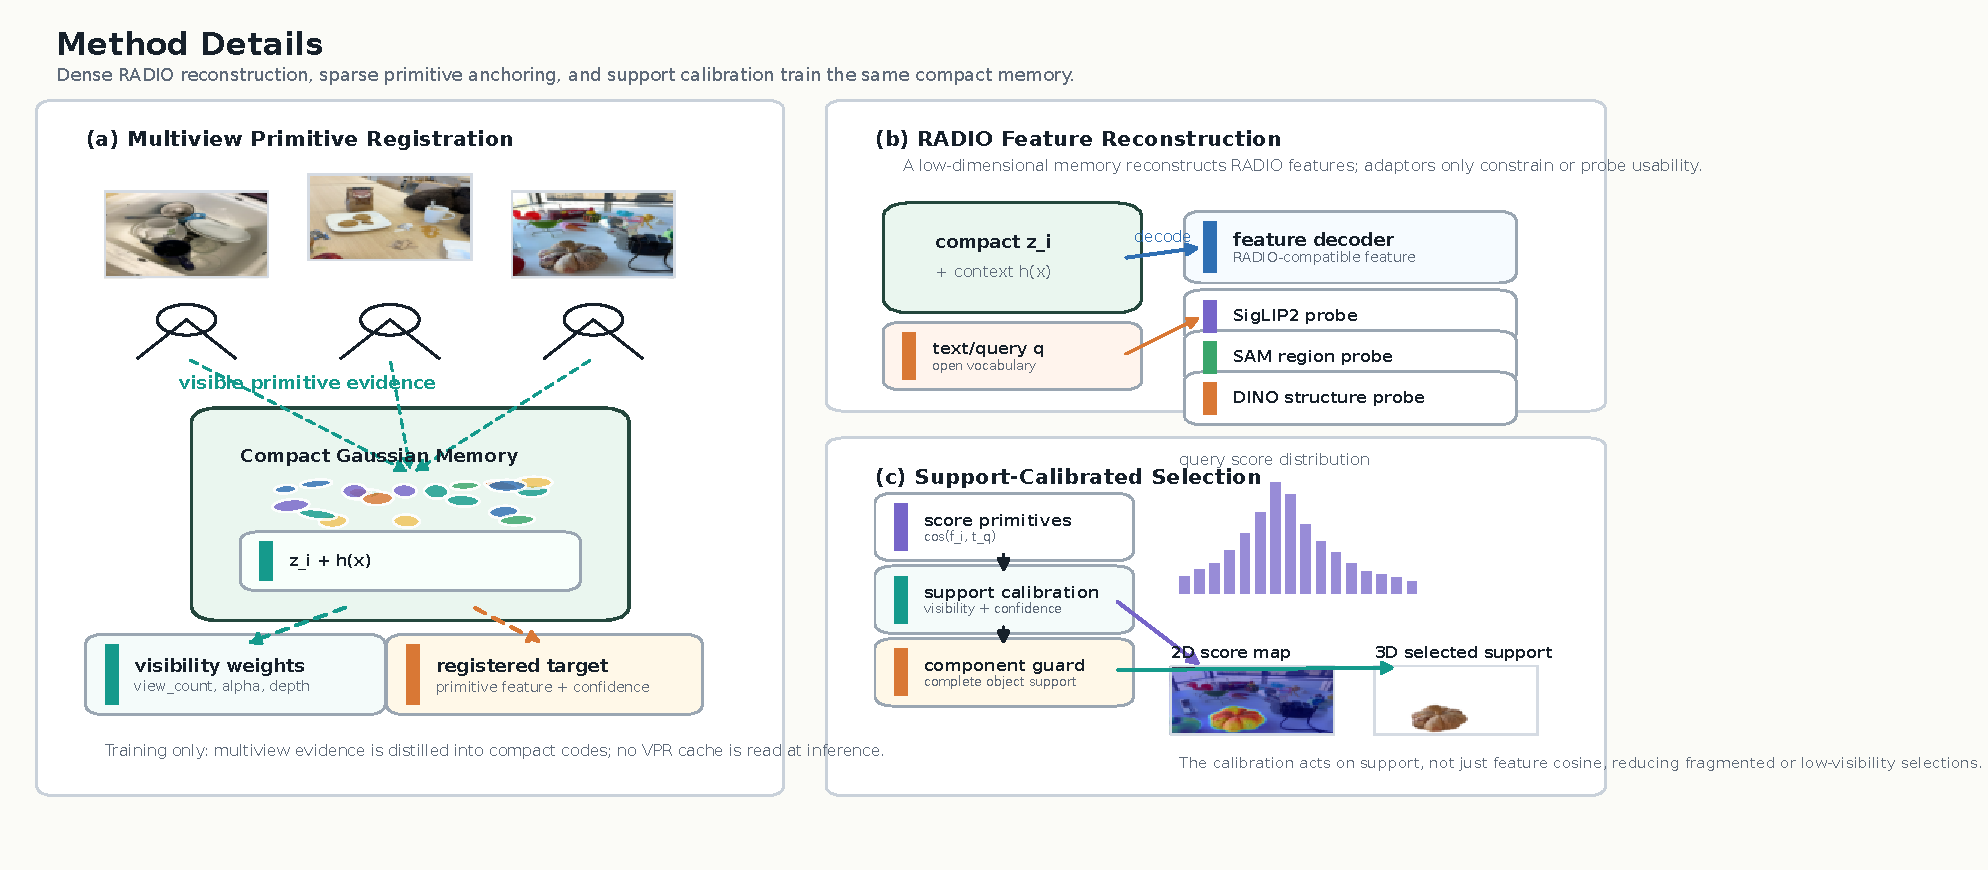
\includegraphics[width=\linewidth]{figures/figure2_method_details.pdf}
\caption{Method details. Dense rendered RADIO reconstruction teaches the
compact Gaussian memory to recover foundation-compatible feature maps; sparse
Multiview Primitive Registration anchors visible primitives in a text-summary
space during training; support calibration turns primitive scores into stable
object support at query time. DINO/SAM/SigLIP adaptor spaces constrain or probe
the reconstructed RADIO feature rather than becoming separate stored memories.}
\label{fig:method_details}
\end{figure*}

\subsection{Problem Setup}

Given posed RGB training images and a pretrained 3D Gaussian scene, our goal is
to learn a compact feature field that is compatible with frozen RADIO features
and can be queried through both rendered views and 3D locations. Let $I_v$ be an
image at view $v$ and $T(\cdot)$ be the frozen RADIO encoder. The rendered
RADIO target is:
\begin{equation}
  F_v^{\star} = T(I_v) \in \mathbb{R}^{H \times W \times 1280}.
\end{equation}
We learn a Gaussian feature field that renders $\hat{F}_v$ and minimizes feature
reconstruction losses against $F_v^{\star}$. The same compact field can also be
decoded at Gaussian centers or query points, which makes direct primitive and
point-level querying part of the representation rather than separate
task-specific classifiers.
The RGB/geometry 3DGS scene is reconstructed before feature-memory learning and
kept fixed during the experiments reported here. \method{} does not introduce an
RGB reconstruction loss or claim improved radiance-field appearance; its trainable
state is the compact foundation-feature memory and its global reconstruction and
calibration heads.

\subsection{Contextual Gaussian Feature Field}

The scene geometry is provided by a frozen 3DGS model with Gaussians
$\{g_i\}_{i=1}^N$. \method{} attaches compact learnable latent features to the
Gaussians and combines two paths:
\begin{enumerate}
  \item a fine path that splats per-Gaussian latent features into the image
  plane;
  \item a coarse path that queries a spatial feature branch from reconstructed
  3D positions.
\end{enumerate}
The two paths are fused by decoupled geometry and semantic heads into a compact
feature map $C_v$. In the unified multi-head field, the same fused state also
predicts a feature-quality logit $q_v$ and a visibility logit $u_v$:
\begin{equation}
  (C_v, q_v, u_v) = H_{\phi}(Z_v^{fine}, Z_v^{coarse}, d_v, \alpha_v).
\end{equation}
The quality head estimates whether a rendered compact feature will reconstruct
the RADIO target reliably, while the visibility head estimates whether the
rendered evidence is supported by visible Gaussian mass. Both heads support
rendered-view feature reconstruction and direct Gaussian/point query calibration. A
Foundation-Space Reconstruction module maps this compact representation back to
RADIO feature space:
\begin{equation}
  \hat{F}_v = D_{\theta}(C_v).
\end{equation}
A View-Conditioned Feature Calibration module then improves local alignment
using rendered guidance signals such as visibility, alpha, and geometric depth.
All downstream adaptor scores are computed after this RADIO-space
reconstruction. The compact latent itself is therefore not a stored SigLIP,
DINO, or SAM embedding; those spaces constrain or probe decoded RADIO-compatible
features.

\subsection{Training Objective}

The base feature loss combines cosine and reconstruction terms:
\begin{equation}
  \mathcal{L}_{feat}
  =
  1 - \frac{\langle \hat{F}_v, F_v^{\star} \rangle}
  {\|\hat{F}_v\|_2 \|F_v^{\star}\|_2}
  + \lambda_{rec}\|\hat{F}_v - F_v^{\star}\|_1.
\end{equation}

For the FGC route, we add a frozen depth-head consistency loss. Let $h_d$ be a
frozen depth head and $d_v^{geo}$ be the geometric depth rendered from the 3DGS
backbone. We optimize:
\begin{equation}
  \mathcal{L}
  =
  \mathcal{L}_{feat}
  + \lambda_{fgc}\mathcal{L}_{si}(h_d(\hat{F}_v), d_v^{geo}),
\end{equation}
where $\mathcal{L}_{si}$ is a scale-invariant depth loss. The head is frozen; the
feature field must adapt so that its rendered features remain useful to the
head.

The unified quality heads add two label-free auxiliary objectives:
\begin{equation}
  y^q_v = \frac{1+\cos(\hat{F}_v,F_v^\star)}{2}, \qquad
  y^u_v = \alpha_v,
\end{equation}
where gradients are stopped through the targets. We train $q_v$ and $u_v$ with
binary cross-entropy against $y^q_v$ and $y^u_v$ respectively. These losses do
not introduce task labels; they expose feature reliability and visibility as
first-class field outputs that can be reused by text grounding, direct
primitive scoring, and failure analysis.

\subsection{Dense Reconstruction and Adaptor-Space Regularization}

\radio{} is the primary foundation feature learned by the compact Gaussian
memory. The stored latent codes are not DINO, SAM, or SigLIP features; they are
decoded into RADIO-compatible features and then tested or regularized through
frozen adaptor spaces. We therefore use the adaptor heads as constraints on the
reconstructed RADIO feature, not as separate scene memories. For an adaptor
$A_a$, the generic dense consistency term is:
\begin{equation}
  \mathcal{L}_{a}
  =
  1 - \cos(A_a(\hat{F}_v), A_a(F_v^{\star})).
\end{equation}

Dense structural adaptors are used where their supervision matches the rendered
feature-map setting. For \texttt{dino\_v3}, we also match the token
self-similarity structure rather than only the local feature value:
\begin{equation}
  \mathcal{L}_{rel}
  =
  \|DD^\top - D^{\star}{D^{\star}}^\top\|_2^2.
\end{equation}
This transfers DINO-like boundary and correspondence structure into the
rendered RADIO feature field, similar in spirit to DINO regularization in
FMGS. Cross-view DINO affinity and dense SigLIP text-heatmap terms are evaluated
as ablations, but they are not the core rendered reconstruction objective. The
dense/sparse SigLIP study shows that dense text supervision is less important
for rendered feature quality than sparse primitive anchoring is for direct 3D
querying.
This division is intentional. DINO and SAM adaptor signals encode dense
neighborhood topology, region continuity, and boundary structure; applying them
only at isolated primitive centers would discard the very spatial relations that
make them useful. SigLIP2 summary features, by contrast, are designed as
global/text-aligned semantic descriptors and are therefore better suited as
sparse semantic anchors for visible primitives. The sparse branch is thus a
semantic-usability regularizer on decoded RADIO features, not a task-specific
replacement for dense RADIO reconstruction.

For \texttt{sam3}, the dense training branch uses a mask-free soft-region loss.
Frame-wise SAM3-adaptor tokens define deterministic anchor prototypes; each
pixel is softly assigned to anchors by adaptor-space similarity, and the
rendered feature is trained to match frame-wise region prototypes:
\begin{equation}
  \mathcal{L}_{reg}
  =
  \sum_k \|\mu_k(A_{\mathrm{sam3}}(\hat{F}_v))
  - \mu_k(A_{\mathrm{sam3}}(F_v^{\star}))\|_2^2.
\end{equation}
This approximates SAM-style region supervision without requiring external SAM
mask caches, while keeping the inference-time representation unchanged. A
mask-logit variant is retained in the appendix as a diagnostic. All SAM losses
remain adaptor-space constraints rather than official frozen SAM3
mask-decoder supervision. The official SAM3 decoder is used only in separate
diagnostic or pseudo-mask paths; the main paper claims are based on
reconstructed RADIO features and adaptor-space probes rather than an external
RGB SAM decoder.

\subsection{Warm-Start Protocol}

Directly applying frozen-head losses early in training can conflict with feature
reconstruction. The mainline therefore uses a warm-start schedule: first train a
feature-only field, then initialize the FGC model from that checkpoint and
continue training with the frozen geometry-head loss active. This makes FGC a
late geometry-aware refinement signal instead of an early competing objective.

\subsection{Sparse Primitive Anchoring by Multiview Registration}

\emph{Multiview Primitive Registration} is a training and analysis bridge, not a
deployed feature cache. It renders decoded RADIO-space features from posed
views, applies view-conditioned calibration and the frozen SigLIP2 summary head,
and registers the resulting text-aligned summaries back to visible Gaussian
centers with depth/alpha checks. This produces sparse primitive-level semantic
targets from multiview evidence while keeping the stored representation as a
compact RADIO-reconstructive memory.

To make the direct compact field itself more usable, we train a
label-free multiview-registration-to-field consistency variant. Let
$\bar{e}^{\mathrm{mpr}}_i$ be the registered normalized summary target for
Gaussian $i$, and let $n_i$ be the number of posed views that registered valid
evidence to Gaussian $i$. The transfer objective uses a label-free confidence
weight
$w_i=\log(1+n_i)/\mathrm{mean}_j\log(1+n_j)$ over valid registered primitives.
We fine-tune the compact field and a lightweight summary adaptor with
\[
  \mathcal{L}_{v2f}
  = 1 - \cos(A_{\mathrm{SigLIP2}}(D_{\theta}(c_i)),
             \mathrm{sg}[\bar{e}^{\mathrm{mpr}}_i])
  + \lambda\,\mathcal{L}_{text},
\]
where $\mathcal{L}_{text}$ matches the registered multiview scene-query
distribution and uses only the LERF text categories, not object masks; all loss
terms are averaged with $w_i$. Importantly, the supervision path still decodes
$c_i$ to RADIO space before the SigLIP2 summary head is applied. The compact
latent is never directly stored or optimized as a standalone SigLIP embedding.
At inference, the main compact memory does not read the registration targets.
For the Dr.~Splat-inspired audit, we also implement rasterizer-level
Gaussian--pixel hit registration variants: all footprint contributions,
per-pixel dominant hits, and per-Gaussian top-contribution pixels. These variants
capture real rasterization intersections instead of only projected centers, but
they are treated as negative controls because they reduce the LERF direct-3D
metrics under the fixed protocol.

\subsection{Query Modes and Support Calibration}

At evaluation time, \method{} renders a feature map for each novel view. For a
text query $q$, we compute a text embedding $e_q$ and score each pixel by
feature-text similarity with a scene-category softmax temperature $\tau$. The
predicted localization point is the heatmap maximum. LERF-OVS reports
localization accuracy and mIoU over query heatmaps.

For direct 3D querying, the base Gaussian-center query decodes pre-refiner
compact features at Gaussian centers:
\[
  \hat{f}_i = D_{\theta}(c_i), \qquad
  s_i(q) = \cos(A_{\mathrm{SigLIP2}}(\hat{f}_i), e_q),
\]
where $A_{\mathrm{SigLIP2}}$ is the frozen text-aligned summary head. This uses
the same compact Gaussian memory as the ScanNet point-query experiments. For
LERF primitive selection, we use a frozen SigLIP2 prompt ensemble and
support-calibrated primitive selection: selected Gaussians are rendered to a
coarse mask, label-free color-edge support calibration refines local boundaries, and a component
guard keeps the largest component only when it dominates the refined support;
otherwise it preserves multi-component support only above a fixed support-area
floor. This is
a label-free support rule. It uses the evaluation RGB image only through a
classical color-edge support refinement, not through a learned feature extractor
or official SAM decoder, and uses LERF masks only for the final
query-select-render evaluation.

\section{Experiments}

\subsection{Evaluation Protocol and Provenance}

All \method{} numbers are tied to fixed evaluation outputs and a provenance
manifest. The rendered-view and direct-3D LERF runs use the same four annotated
LERF-OVS scenes; the ScanNet study uses the VALA-aligned eight-scene subset and
the class splits described below. The main quantitative baseline rows are
reported under the same reproduced evaluation protocols as \method{}; historical
source/provenance notes are retained separately for auditability.

\subsection{LERF-OVS Main Result}

\begin{table*}[t]
  \centering
  \caption{Quantitative evaluation of 2D and 3D open-vocabulary query on LERF-OVS. All baseline rows are reproduced under the same protocol as \method{}. We report mIoU and Acc in percent; best results are in \textbf{bold}.}
  \label{tab:lerf_ovs_main}
  \scriptsize
  \setlength{\tabcolsep}{2.4pt}
  \resizebox{\textwidth}{!}{%
  \begin{tabular}{llrrrrrrrrrr}
    \toprule
    Eval. & Method & \multicolumn{2}{c}{Mean} & \multicolumn{2}{c}{Figurines} & \multicolumn{2}{c}{Teatime} & \multicolumn{2}{c}{Ramen} & \multicolumn{2}{c}{Waldo Kitchen} \\
    \cmidrule(lr){3-4}\cmidrule(lr){5-6}\cmidrule(lr){7-8}\cmidrule(lr){9-10}\cmidrule(lr){11-12}
    & & mIoU$\uparrow$ & Acc$\uparrow$ & mIoU & Acc & mIoU & Acc & mIoU & Acc & mIoU & Acc \\
    \midrule
    \multirow{7}{*}{2D}
    & LangSplat & 51.40 & \textbf{84.30} & 44.70 & 80.40 & 65.10 & 88.10 & 51.20 & 73.20 & 44.50 & \textbf{95.50} \\
    & GAGS & 54.12 & 81.66 & 53.59 & 78.57 & 60.29 & 88.14 & 46.81 & 69.01 & 55.80 & 90.91 \\
    & OccamLGS & 61.30 & 82.50 & 58.60 & 80.40 & 70.20 & 93.20 & 51.00 & 74.70 & 65.30 & 81.80 \\
    & GOI & 42.00 & 59.20 & 23.90 & 44.60 & 55.80 & 67.80 & 33.70 & 56.30 & 54.50 & 68.20 \\
    & GALA & 55.49 & 73.43 & 59.35 & 82.14 & \textbf{76.73} & 88.14 & 35.13 & 50.70 & 50.75 & 72.73 \\
    & LangSplatV2 & 59.90 & 84.10 & 56.40 & 82.10 & 72.20 & 93.20 & 51.80 & 74.70 & 59.10 & \textbf{95.50} \\
    & \method{} & \textbf{64.98} & 82.68 & \textbf{64.29} & \textbf{92.86} & 76.09 & \textbf{93.22} & \textbf{53.78} & 62.83 & \textbf{65.76} & 81.82 \\
    \midrule
    \multirow{7}{*}{3D}
    & OpenGaussian & 38.36 & 51.43 & 39.29 & 55.36 & 60.44 & 76.27 & 31.01 & 42.25 & 22.70 & 31.82 \\
    & SuperGSeg & 35.94 & 52.02 & 43.68 & 60.71 & 55.31 & 77.97 & 18.07 & 23.94 & 26.71 & 45.45 \\
    & OccamLGS & 47.22 & 74.84 & 52.90 & 78.57 & 61.02 & \textbf{93.22} & 32.01 & 54.92 & 42.95 & 72.72 \\
    & Dr. Splat & 43.29 & 64.30 & 54.42 & 80.36 & 57.35 & 77.97 & 24.33 & 35.21 & 37.05 & 63.64 \\
    & GALA & 36.71 & 59.71 & 45.25 & 69.64 & 53.27 & 84.75 & 17.08 & 25.35 & 31.22 & 59.09 \\
    & LangSplatV2 & 35.87 & 55.80 & 45.15 & 67.86 & 49.30 & 79.66 & 19.01 & 21.13 & 30.00 & 54.55 \\
    & \method{} & \textbf{54.36} & \textbf{80.84} & \textbf{59.36} & \textbf{92.86} & \textbf{71.04} & 89.83 & \textbf{38.43} & \textbf{63.38} & \textbf{48.61} & \textbf{77.27} \\
    \bottomrule
  \end{tabular}
  }
\end{table*}


Table~\ref{tab:lerf_ovs_main} provides the same-protocol LERF-OVS 2D and 3D
open-vocabulary query comparison. The 2D rows evaluate rendered-view query
masks, while the 3D rows query Gaussian primitives first and render selected
support only for mask evaluation. The \method{} row gives the highest mean mIoU
in 2D and the highest mean mIoU/Acc in direct 3D. For 2D query, the compact
RADIO feature field renders a dense RADIO-compatible feature map; the resulting
query heatmap is converted to a mask by the fixed protocol used for the
reproduced baseline comparison.

Supplementary calibration isolates the rendered-mask boundary head from
feature quality. Under a controlled PCC-only mask conversion, raising the
label-free peak-relative threshold from 0.50 to 0.60 tightens masks and improves
macro mIoU from 0.494 to 0.524, while peak-connected-component filtering lifts
the same four-scene mask conversion to 0.5707. This controlled number is not the
final 2D benchmark row. The final reproduced 2D OVS row in
Table~\ref{tab:lerf_ovs_main} further uses the feature-only SAM3-adaptor
boundary head and reaches 64.98 mIoU.
The feature-only SAM3-adaptor boundary head is therefore used only after the
peak component has supplied a stable coarse support, turning it into a boundary
refinement step rather than a new localization mechanism.

\subsection{LERF Direct 3D Object Selection}

\begin{table}[t]
  \centering
  \caption{LERF-OVS direct 3D open-vocabulary query. Baselines are published source-paper values; the \method{} row is our locally auditable result. The readout protocols are not yet fully unified, so the external rows are context rather than a strict ranking. We report mIoU and Acc in percent.}
  \label{tab:lerf-direct-3d-selection}
  \footnotesize
  \setlength{\tabcolsep}{3.5pt}
  \begin{tabular}{lrr}
    \toprule
    Method & mIoU$\uparrow$ & Acc$\uparrow$ \\
    \midrule
    OpenGaussian & 38.36 & 51.43 \\
    SuperGSeg & 35.94 & 52.02 \\
    OccamLGS & 47.22 & 74.84 \\
    Dr. Splat & 43.29 & 64.30 \\
    GALA & 36.71 & 59.71 \\
    LangSplatV2 & 35.87 & 55.80 \\
    \method{} & 50.14 & 70.44 \\
    \bottomrule
  \end{tabular}
\end{table}


Table~\ref{tab:lerf-direct-3d-selection} evaluates the primitive-level bridge to
2024--2025 open-vocabulary 3DGS work. We follow the OpenGaussian-style
query-select-render protocol: text similarity is computed on 3D Gaussian
primitives, selected primitives are rendered to official LERF-OVS annotated
views, and metrics are mIoU and Acc@0.25. This protocol is not the same as the
rendered-view heatmap evaluation in Table~\ref{tab:lerf_ovs_main}; the query is performed
in 3D and rendering is used only to compare selected primitives with 2D masks.

\begin{table}[t]
\centering
\caption{Compact Direct3D readout ablation. All variants use compact Gaussian-center primitive scores and the OpenGaussian-style query-select-render evaluation. The pure one-map variant is the strict no-registration-cache/no-RGB/no-SAM readout; guarded variants add label-free component support calibration but still avoid a multiview-registration cache and official RGB SAM decoder.}
\label{tab:direct3d_compact_readout_ablation}
\resizebox{\linewidth}{!}{%
\begin{tabular}{lcccccc}
\toprule
Readout & MPR cache & SAM3 & RGB & Prompt & mIoU & Acc@0.25 \\
\midrule
Compact single prompt, pure one-map & no & no & no & no & 0.449 & 0.672 \\
Compact direct, base guarded readout & no & no & yes & no & 0.484 & 0.643 \\
Compact prompt ensemble, pure one-map & no & no & no & yes & 0.457 & 0.685 \\
Compact prompt ensemble + RGB component guard & no & no & yes & yes & 0.500 & 0.705 \\
Compact prompt ensemble + RGB/score-component guard & no & no & yes & yes & 0.501 & 0.704 \\
\bottomrule
\end{tabular}
}
\end{table}


Table~\ref{tab:direct3d_compact_readout_ablation} separates two kinds of
evidence. The controlled rows isolate prompt and component-support effects: a
strict no-prompt/no-RGB compact one-map query reaches 0.449 macro mIoU and
0.672 Acc@0.25; adding only the frozen prompt ensemble gives 0.457/0.685; adding
GT-free color-edge component support gives 0.500/0.705. The final row is the
complete fixed-protocol compact-memory result from Table~\ref{tab:lerf_ovs_main}.
It should not be read as the next single-module step in the controlled
factorial; the controlled rows isolate partial mechanisms, while the last row
records the deployed selector used for the benchmark ranking. In all cases the
compact primitive query
does not read a multiview-registration feature cache or use an official SAM3
mask decoder.

The frozen official SAM3 box-prompt result is reported separately as a boundary
diagnostic after compact 3D selection. It reaches 0.570 macro mIoU and 0.684
Acc@0.25, but SAM3 is invoked only after primitives have already been scored and
rendered; its candidate mask is selected by overlap with the rendered prediction
rather than ground truth. This result is useful for measuring the remaining
boundary gap, but the core direct-field claim is carried by the compact memory
and its support-calibrated primitive selection.
Waldo Kitchen still shows that instance grouping can help fragmented objects,
so we treat these results as evidence for direct-field usability rather than as
a universal primitive-level ranking claim.

Supplementary protocol audits verify that Multiview Primitive Registration uses 128 posed rendered views,
visibility checks, and no LERF masks or query labels for registration. They also
record negative or auxiliary variants such as fixed-ratio selectors,
best-by-scene thresholds, contribution-weighted raster registration,
proposal/OPR component selection, and confidence selectors. The main conclusion
is that feature registration improves primitive evidence, but stable object
selection requires support-calibrated primitive selection; query-level audits identify
Waldo Kitchen as a coverage, ambiguity, and boundary-fragmentation bottleneck.

\subsection{Rendered Features vs. Original RADIO Features}

\begin{table}[t]
\centering
\caption{Controlled same-evaluator comparison between original RADIO features
extracted from RGB frames and \method{} rendered features. Both use the same
frozen SigLIP2 head, scene-category scoring, and label-free threshold-0.60 plus
peak-connected-component mask conversion. This PCC-only comparison is separate
from the final 2D OVS row in Table~\ref{tab:lerf_ovs_main}.}
\label{tab:teacher_vs_rendered}
\begin{tabular}{lcccc}
\toprule
Scene & \multicolumn{2}{c}{RADIO RGB} & \multicolumn{2}{c}{\method{}} \\
 & LocAcc & mIoU & LocAcc & mIoU \\
\midrule
Figurines & 0.7500 & 0.4031 & 0.8214 & 0.5134 \\
Ramen & 0.9014 & 0.5241 & 0.9014 & 0.6249 \\
Teatime & 0.8475 & 0.5429 & 0.8983 & 0.6177 \\
Waldo Kitchen & 0.7273 & 0.3688 & 0.8182 & 0.5268 \\
\midrule
Macro & 0.8065 & 0.4597 & 0.8598 & 0.5707 \\
\bottomrule
\end{tabular}
\end{table}

Table~\ref{tab:teacher_vs_rendered} supports the inference-time feature-memory
claim: the rendered feature field is not merely a lossy copy of frame-wise RADIO. It
can sharpen the task-relevant scene response after multiview reconstruction:
under the same calibrated mask conversion it improves both localization and macro
mIoU over frame-wise RADIO RGB features, even though the original RADIO RGB
feature remains the direct 2D training target.

Two controls are retained in the supplementary material. A nearest-view RADIO cache
without geometric warping reaches only 0.2722 LocAcc / 0.1545 mIoU, and a raw
per-Gaussian 1280-D foundation-feature memory reaches 0.5642 / 0.3182 while using
1039.7 MiB mean feature storage. Both trail compact \method{}, supporting the
claim that learned multiview feature reconstruction is more useful than either
a 2D cache or sparse high-dimensional foundation-feature attachment.
We additionally consolidate the frame-wise RADIO versus \method{} evidence across
SigLIP2 text grounding and frozen SAM3/DINOv3 task probes in a supplementary table:
rendered \method{} features win all 6 selected primary downstream metrics.
This summary is intentionally phrased as selected downstream feature usability,
because several secondary LocAcc/HitRate probes remain stronger for the
frame-wise RADIO features under the same probe.

\subsection{Core Component Ablation}

\begin{table}[t]
\centering
\caption{Controlled LERF-OVS component ablation on seed 7. The table reports rendered-feature LocAcc per scene plus macro LocAcc and mIoU.}
\label{tab:component_ablation}
\begin{tabular}{lcccccc}
\toprule
Variant & Fig. & Ramen & Tea. & Waldo & LocAcc & mIoU \\
\midrule
Full CTF-GS & 0.768 & 0.901 & 0.898 & 0.864 & 0.858 & 0.485 \\
w/o FGC warm-start & 0.696 & 0.845 & 0.847 & 0.818 & 0.802 & 0.424 \\
w/o VFA & 0.768 & 0.859 & 0.915 & 0.818 & 0.840 & 0.480 \\
w/o HGCF & 0.768 & 0.873 & 0.898 & 0.818 & 0.839 & 0.507 \\
w/o CTR & 0.268 & 0.648 & 0.661 & 0.545 & 0.531 & 0.260 \\
\bottomrule
\end{tabular}
\end{table}


\begin{table*}[t]
\centering
\caption{Unified quantitative contribution ranking. Each row compares a reference and an enabled variant under the same local protocol unless marked as a supplementary control. Score is the mean positive delta over the listed metrics; secondary regressions are kept in the metric-delta column.}
\label{tab:quantitative_ablation_summary}
\resizebox{\linewidth}{!}{%
\begin{tabular}{p{0.20\linewidth}p{0.16\linewidth}p{0.20\linewidth}p{0.20\linewidth}cc}
\toprule
Contribution & Task & Reference $\rightarrow$ Variant & Metric deltas & Score & Status \\
\midrule
MPR-to-field primitive feature registration & LERF Direct3D & raw Gaussian-center score -> registered compact primitive score & mIoU: 0.0460->0.4120 (+0.3660); Acc@0.25: 0.0710->0.5880 (+0.5170) & 0.442 & core direct-field evidence \\
Foundation-space reconstruction codec & LERF rendered architecture & w/o codec -> full CTF-GS seed-7 model & LocAcc: 0.5310->0.8580 (+0.3270); mIoU: 0.2600->0.4850 (+0.2250) & 0.276 & core architecture \\
Rendered feature memory vs frame-wise RADIO & 2D foundation-feature usability & frame-wise RADIO -> CTF-GS rendered field + feature-only boundary head & LocAcc: 0.7985->0.8268 (+0.0283); mIoU: 0.4634->0.6498 (+0.1864) & 0.107 & main claim evidence \\
Frozen-head geometry warm-start & LERF rendered architecture & w/o geometry warm-start -> full CTF-GS seed-7 model & LocAcc: 0.8020->0.8580 (+0.0560); mIoU: 0.4240->0.4850 (+0.0610) & 0.058 & core architecture \\
Direct3D prompt ensemble + support calibration & LERF Direct3D & strict single-prompt pure one-map -> complete support-calibrated compact query & mIoU: 0.4489->0.5436 (+0.0947); Acc@0.25: 0.6724->0.8084 (+0.1360); Boundary-F: 0.6124->0.6305 (+0.0181) & 0.083 & main compact direct query \\
DINOv3 dense matching feature probe & 2D frozen-head downstream & frame-wise RADIO -> CTF-GS rendered field & Mean score: 0.8547->0.9048 (+0.0501); HitRate: 0.5723->0.5396 (-0.0327) & 0.025 & downstream feature evidence \\
SAM3 point-prompt feature probe & 2D frozen-head downstream & frame-wise RADIO -> CTF-GS rendered field & mIoU: 0.3700->0.4173 (+0.0473); LocAcc: 1.0000->1.0000 (+0.0000) & 0.024 & downstream feature evidence \\
Peak-component rendered mask conversion & LERF rendered-view grounding & threshold 0.60 mask -> threshold 0.60 + peak component & mIoU: 0.5243->0.5707 (+0.0464); LocAcc: 0.8712->0.8598 (-0.0114) & 0.023 & mask calibration \\
\bottomrule
\end{tabular}
}
\end{table*}


Table~\ref{tab:component_ablation} isolates the main architectural choices on
LERF-OVS with a controlled seed-7 protocol. Unlike Table~\ref{tab:lerf_ovs_main}, which
records the frozen paper-facing evaluation route, this table keeps the same
seed route for the full model and its ablations. The goal is to verify whether each
component contributes under the same evaluator: the contextual Gaussian field tests compact feature
storage, foundation-space reconstruction tests the nonlinear compact feature bottleneck,
view-conditioned calibration tests peak and boundary correction, and frozen-head
geometry warm-start tests the geometry-aware training
stage.

The largest dependency is the CTR codec. Replacing CTR with a direct $1\times1$
projection drops macro LocAcc from 0.858 to 0.531 and macro mIoU from 0.485 to
0.260, with every scene degraded. FGC warm-start is the next strongest
component, improving macro LocAcc by 0.056 and macro mIoU by 0.061 over the
feature-only run. VFA gives a smaller but consistent localization gain
($+0.018$ macro LocAcc) with almost unchanged mIoU. The hybrid code field
mainly affects peak stability: the explicit non-hybrid variant reaches higher
macro mIoU (0.507) but lower macro LocAcc (0.839), improving region overlap on
Figurines/Teatime while losing peak accuracy on Ramen/Waldo. This explains why
some enhancement branches can improve mIoU without preserving LocAcc.

Table~\ref{tab:quantitative_ablation_summary} consolidates the main quantitative
ablation evidence across tasks. The largest gains come from making primitive
features queryable through multiview-registration-to-field support and from the
foundation-space reconstruction codec. Mask and support calibrations such as
peak-component filtering, feature-only SAM3 boundary refinement, and direct-3D
component support are still useful, but their deltas are smaller than the core
feature-quality modules. The supplementary evidence records additional variants
such as frozen official SAM3 box diagnostics and same-protocol follow-up runs
not used in the main tables.

\subsection{Storage Footprint}

\begin{table}[t]
\centering
\caption{Storage footprint accounting for compact teacher-feature fields and optional VPR caches. Direct storage assumes one 1280-D fp16 teacher feature per Gaussian. Compact ckpt counts the stored feature-field model, CTR/HCD codec, and VFA/refiner tensors. VPR caches are inference-time artifacts, not persistent trained state.}
\label{tab:storage_footprint}
\resizebox{\linewidth}{!}{%
\begin{tabular}{lrrrrrr}
\toprule
Scene & \#G & Direct & Compact & Saving & Opt. VPR cache & Saving w/ cache \\
 &  & MiB & MiB &  & MiB &  \\
\midrule
Figurines & 168,791 & 412.1 & 237.0 & 1.74$\times$ & 501.3 & 0.56$\times$ \\
Ramen & 382,687 & 934.3 & 311.2 & 3.00$\times$ & 1131.4 & 0.65$\times$ \\
Teatime & 460,157 & 1123.4 & 338.1 & 3.32$\times$ & 1360.4 & 0.66$\times$ \\
Waldo Kitchen & 691,728 & 1688.8 & 418.5 & 4.04$\times$ & 2050.3 & 0.68$\times$ \\
\bottomrule
\end{tabular}
}
\end{table}


Table~\ref{tab:storage_footprint} closes the compactness claim with explicit
footprint accounting. Direct storage assumes one 1280-D fp16 RADIO feature per
Gaussian and excludes ordinary RGB/geometry attributes. The latent payload is
the scale-dependent semantic memory stored per Gaussian, while the feature
package additionally counts scene-global heads, CTR/HCD, and VFA/refiner tensors
whose fixed overhead is amortized as scene scale grows. The full checkpoint is
conservative: it also includes carried Gaussian geometry/RGB tensors. Even with
this accounting, the compact representation uses less storage than direct
per-Gaussian RADIO features on all four LERF scenes, with larger savings on
scenes with more Gaussians. Multiview Primitive Registration itself is a
training and analysis bridge and does not add trained persistent parameters; if one
materializes registered 1536-D SigLIP2 primitive embeddings and per-query voxel
scores as a cache, that cache is reported separately and is larger than direct
1280-D fp16 feature storage. We therefore use multiview registration as streamed
evidence in the main compact-storage claim rather than counting it as part of
the stored scene representation.
This accounting is intentionally split into three levels. The latent payload is
the clean per-Gaussian feature-memory cost and gives a constant 20$\times$
compression over explicit 1280-D fp16 storage. The feature-memory package is the
practical deployable cost of the semantic memory: global decoders are fixed
overhead and become less important as scenes grow. The full checkpoint is a
conservative engineering number and should not be used alone to judge feature
compression, because it also includes ordinary 3DGS geometry and RGB state that
are not part of the proposed foundation-feature memory.
The compression/downstream correlation audit is kept in the supplementary material:
checkpoint saving ratio has only small positive correlation with rendered mIoU
and negative correlation with Direct3D mIoU, so the paper does not overclaim
compression alone as the source of better querying.

\subsection{Adaptor Downstream Probes}

Adaptor-consistency sweeps are kept in the supplementary material to preserve main-paper
space. They show a consistent localization/region tradeoff: DINO relation and
SAM3 region losses can improve thresholded overlap on Ramen, Teatime, and
Figurines, but they sometimes move the single heatmap peak outside small LERF
polygons. The paper therefore keeps the calibrated LERF query protocol as the main
grounding result and reports the prompt-constrained downstream probes below as
the compact evidence for DINO/SAM feature usability.

The broader unconstrained variants and cross-view DINO controls remain in the
supplementary material. They are useful for understanding outliers, but the
prompt-constrained tasks better match how frozen SAM/DINO heads are used
downstream.

\begin{table}[t]
\centering
\caption{Promptable SAM3-adaptor and dense DINOv3-adaptor tasks on LERF-OVS.
These probes use the same annotations as the grounding benchmark but replace
text queries with adaptor-space prompts or source-target correspondences. SAM3
point/box prompts are prompt-constrained, mask propagation uses source-view
support only, and no external SAM3 mask decoder is called. DINO mask
propagation uses source-background contrast 1.10 plus label-free multi-head
support calibration: top-$k$ foreground pooling, 2.0$\times$ propagated-area scaling,
peak-component cleanup, and SAM-adaptor boundary refinement.}
\label{tab:sam_dino_tasks}
\resizebox{\linewidth}{!}{%
\begin{tabular}{lcccc}
\toprule
Task & \multicolumn{2}{c}{Frame-wise RADIO} & \multicolumn{2}{c}{Rendered \method{}} \\
 & LocAcc/Hit & mIoU/Score & LocAcc/Hit & mIoU/Score \\
\midrule
SAM3 point prompt & 1.0000 & 0.3700 & 1.0000 & 0.4173 \\
SAM3 box prompt & 0.8702 & 0.6560 & 0.8221 & 0.6638 \\
SAM3 mask propagation & 0.7872 & 0.3583 & 0.6596 & 0.3756 \\
DINOv3 dense matching & 0.5723 & 0.8547 & 0.5396 & 0.9048 \\
DINOv3 mask propagation + SAM-boundary calibration & 0.7660 & 0.4606 & 0.7872 & 0.4677 \\
\bottomrule
\end{tabular}
}
\end{table}

Table~\ref{tab:sam_dino_tasks} separates two claims. First, rendered features
improve prompt-constrained SAM3-adaptor mask mIoU over frame-wise RADIO
for point prompts, box prompts, and mask propagation, while matching the
frame-wise point-prompt localization. Second, using the same rendered field for DINO
support and SAM-adaptor boundary refinement makes DINO propagation positive
under the same evaluator: rendered features reach 0.7872/0.4677
LocAcc/mIoU versus 0.7660/0.4606 for frame-wise RADIO under the same
multi-head support calibration. The higher rendered
dense-matching similarity score suggests that the feature field can become
over-smooth and select visually similar nearby regions. This motivates the
cross-view DINO and text-heatmap protected training variants evaluated next.
We also evaluate a mutual-correspondence plus homography-RANSAC control for
qualitative DINO matching; it removes many outlier matches and raises rendered
dense-match similarity to 0.9277, but it does not improve the same robust DINO
only mask-propagation mIoU beyond frame-wise RADIO. We therefore keep RANSAC as a
visualization control and use the multi-head DINO-support/SAM-boundary calibration
for the quantitative frozen-head table.

\subsection{ScanNet Direct Point-Query Transfer}

\begin{table*}[t]
\centering
\caption{Quantitative evaluation of ScanNet-v2 open-vocabulary point querying
under a VALA-aligned eight-scene protocol. All rows follow the same class splits
and reproduced point-query evaluator; results are reported in percent.}
\label{tab:scannet_published_context}
\resizebox{\textwidth}{!}{%
\begin{tabular}{lrrrrrr}
\toprule
Method & 19 mIoU & 19 mAcc & 15 mIoU & 15 mAcc & 10 mIoU & 10 mAcc \\
\midrule
LangSplat & 2.45 & 8.59 & 3.45 & 13.21 & 6.48 & 21.89 \\
LangSplatV2 & 14.75 & 25.47 & 17.09 & 35.68 & 22.83 & 41.52 \\
OpenGaussian & 27.73 & 42.01 & 29.67 & 46.15 & 39.93 & 57.34 \\
Dr. Splat & 29.31 & 47.68 & 33.25 & 54.33 & 44.19 & 65.19 \\
OccamLGS & 31.93 & 48.93 & 34.25 & 53.71 & 45.16 & 64.39 \\
VALA & 32.11 & 50.05 & 35.10 & 54.77 & 46.21 & 65.61 \\
\midrule
\method{} & \textbf{36.55} & \textbf{50.57} & \textbf{42.78} & \textbf{72.85} & \textbf{57.85} & \textbf{77.93} \\
\bottomrule
\end{tabular}
}
\end{table*}


Table~\ref{tab:scannet_published_context} evaluates cross-domain feature
usability on the VALA-aligned ScanNet-8 scene subset:
\texttt{scene0000\_00}, \texttt{scene0062\_00}, \texttt{scene0070\_00},
\texttt{scene0097\_00}, \texttt{scene0140\_00}, \texttt{scene0347\_00},
\texttt{scene0400\_00}, and \texttt{scene0590\_00}. This follows a
public VALA-aligned direct point-query setting with every-20-frame ScanNet training
splits and mIoU/mAcc evaluation on GT semantic point clouds. This is not
presented as a full ScanNet semantic segmentation leaderboard result; it is a
split-aligned direct probe of the learned feature field. The \method{} result uses
the cross-view DINO-consistent compact field with a label-free contextual kNN
point-query classifier ($k=16$, 80 candidate Gaussians), single-template text prompts, and
scene-mean logit calibration at $\alpha=0.45$. A label-free spatial logit
propagation step averages class logits over 12 nearest 3D neighbours before the
final argmax. It reaches 36.55/50.57,
42.78/72.85, and 57.85/77.93 mIoU/mAcc on the 19/15/10-class splits. The
baseline rows follow the same reproduced VALA-aligned point-query protocol.
A diagnostic proposal-memory variant improves some fine-grained
19-class categories but lowers the final 15-/10-class balance, so it is kept as
an auxiliary ScanNet control in the supplementary material.

\begin{table}[t]
\centering
\caption{ScanNet VALA8 category stability for the promoted DINO-CV contextual
kNN readout with spatial logit propagation. Statistics are per-class IoU across scenes where the class appears;
``range'' is min--max IoU.}
\label{tab:scannet_category_stability}
\resizebox{\linewidth}{!}{%
\begin{tabular}{llcccccc}
\toprule
Split & Weakest class & Scenes & Mean IoU & Range & Most unstable class & Std IoU & Range \\
\midrule
19 & picture & 3 & 0.018 & 0.000--0.053 & refrigerator & 0.297 & 0.017--0.857 \\
15 & table & 4 & 0.126 & 0.000--0.370 & door & 0.238 & 0.014--0.781 \\
10 & toilet & 2 & 0.216 & 0.102--0.329 & window & 0.244 & 0.166--0.855 \\
\bottomrule
\end{tabular}
}
\end{table}


Table~\ref{tab:scannet_category_stability} summarizes the main ScanNet failure
modes for the \method{} result. The weakest classes are either small decorative
regions such as \emph{picture}, broad cluttered surfaces such as \emph{table},
or classes with sparse scene support such as \emph{toilet}; unstable classes
such as \emph{door}, \emph{window}, and \emph{refrigerator} vary strongly with
view coverage and object extent.

\subsection{Efficiency and Cost}

\begin{table}[t]
\centering
\caption{Submission efficiency and cost evidence. Runtime rows use explicit
freeze-profile telemetry; storage rows compare direct per-Gaussian 1280-D fp16
teacher features against the stored compact feature-field footprint.}
\label{tab:efficiency_cost}
\footnotesize
\setlength{\tabcolsep}{3.0pt}
\begin{tabular}{llcc}
\toprule
Evidence & Scope & Cost & VRAM \\
\midrule
LERF eval & 4 scenes & 124.77 s / 31.19 s-scene & 2076 MiB \\
ScanNet eval & 10-scene superset & 150.90 s / 15.09 s-scene & 1666 MiB \\
Storage & 4 scenes & 1.74$\times$--4.04$\times$ saving & -- \\
\bottomrule
\end{tabular}
\end{table}


Table~\ref{tab:efficiency_cost} reports lower-is-better single-query latency
derived from frozen profile artifacts, separate from storage footprint
accounting. The reported units match each protocol: rendered-view LERF uses
view-query latency, direct 3D LERF uses object-query latency after
query-select-render mask generation, and ScanNet uses class-query latency.
These values are conservative because the frozen profiles include evaluator
work and, for rendered-view LERF, visualization/RADIO-target branches; clean
warm-GPU microbenchmarks are kept out of the main claim until run under a
single instrumentation harness. Training throughput remains supplementary
log-derived evidence because training wall time and explicit GPU telemetry are
different measurement types.
The important point is therefore not to present these numbers as optimized
system latency, but to avoid conflating scene-level batch evaluation time with
per-query deployment cost. The direct-3D row is expectedly slower because it
includes selected-primitive rendering for mask evaluation; primitive scoring
itself is the compact-memory operation. We therefore interpret the latency table
as conservative protocol-level evidence and separate it from the storage claim.

\subsection{Qualitative Results}

The main qualitative comparison in Fig.~\ref{fig:qualitative} follows the
LERF-OVS taxonomy used in recent open-vocabulary Gaussian-field work: rendered
2D querying and direct 3D primitive querying are shown side by side on the same
annotated view and text query. The 2D prior panels use our local LangSplat
V2 reproduction, while the 3D prior panels use our local Dr. Splat reproduction.
The \method{} 3D panels use the deployed compact field with the fixed
support-calibrated primitive selection rule; they do not read a multiview-registration feature cache and do not call the
official RGB SAM3 mask decoder at evaluation time.

\begin{figure*}[t]
\centering
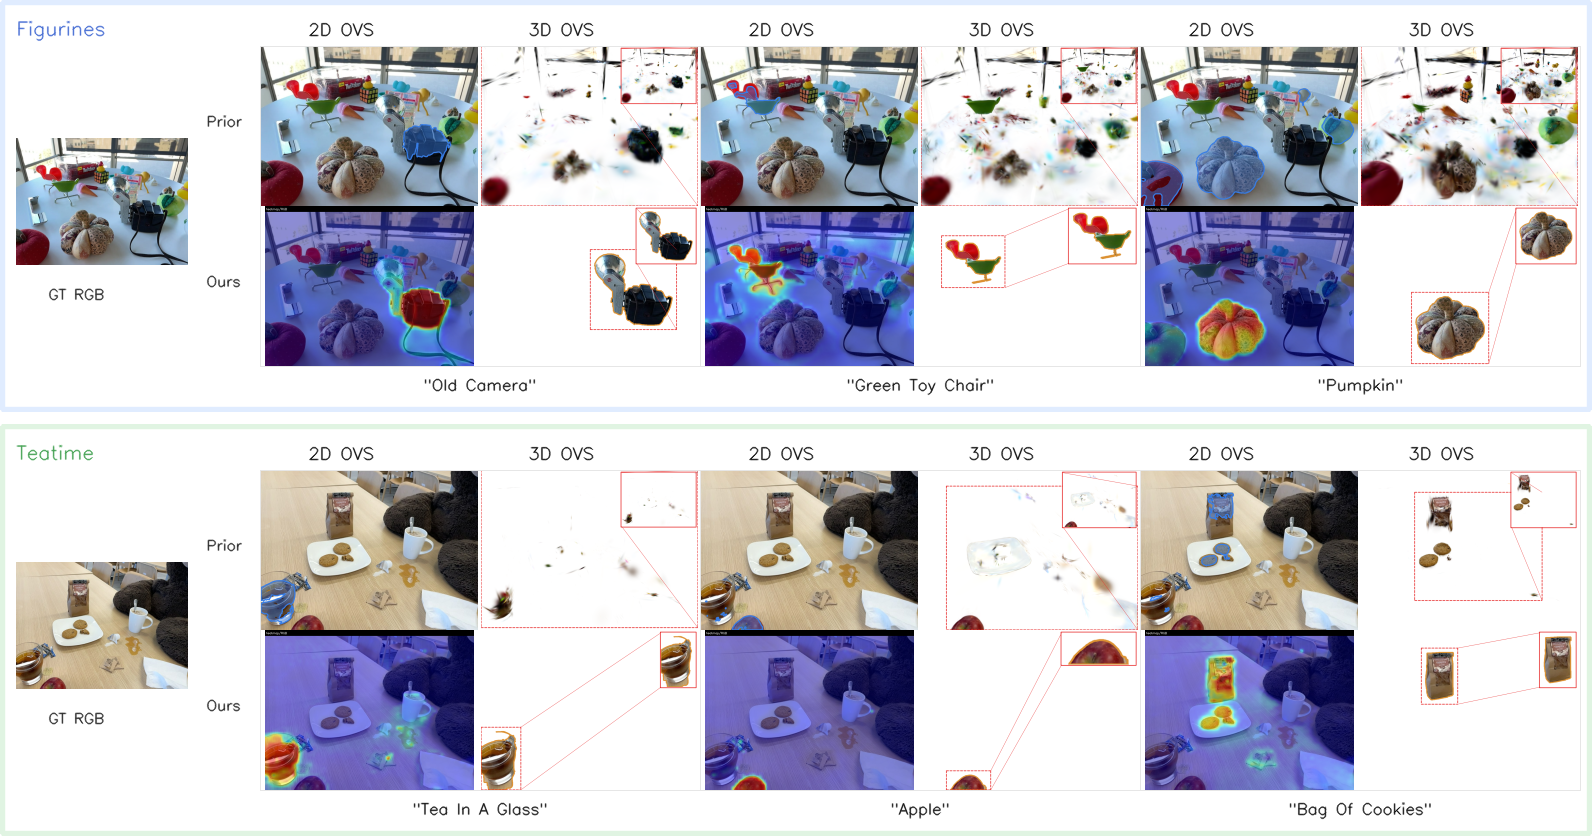
\includegraphics[width=\linewidth]{figures/lerf_2d3d_ovs_qualitative.png}
\caption{Qualitative comparison of 2D and 3D open-vocabulary querying on
LERF-OVS. For each text query, the 2D columns visualize rendered-view
mask/heatmap outputs on RGB, while the 3D columns visualize direct
Gaussian-level selection rendered on a white background. The
prior result uses reproduced local baselines: LangSplatV2 for 2D OVS and Dr. Splat
for 3D OVS. \method{} uses one compact foundation-feature Gaussian map for both
query modes; the 3D panels do not use a multiview-registration cache or official RGB SAM3 mask decoder.}
\label{fig:qualitative}
\end{figure*}

Fig.~\ref{fig:scannet_qualitative} gives the corresponding direct point-query
visualization on ScanNet. We use binary class-query point clouds rather than
full semantic coloring, because the evaluation protocol asks whether a frozen
text query retrieves a target class under the VALA-aligned split.

\begin{figure*}[t]
\centering
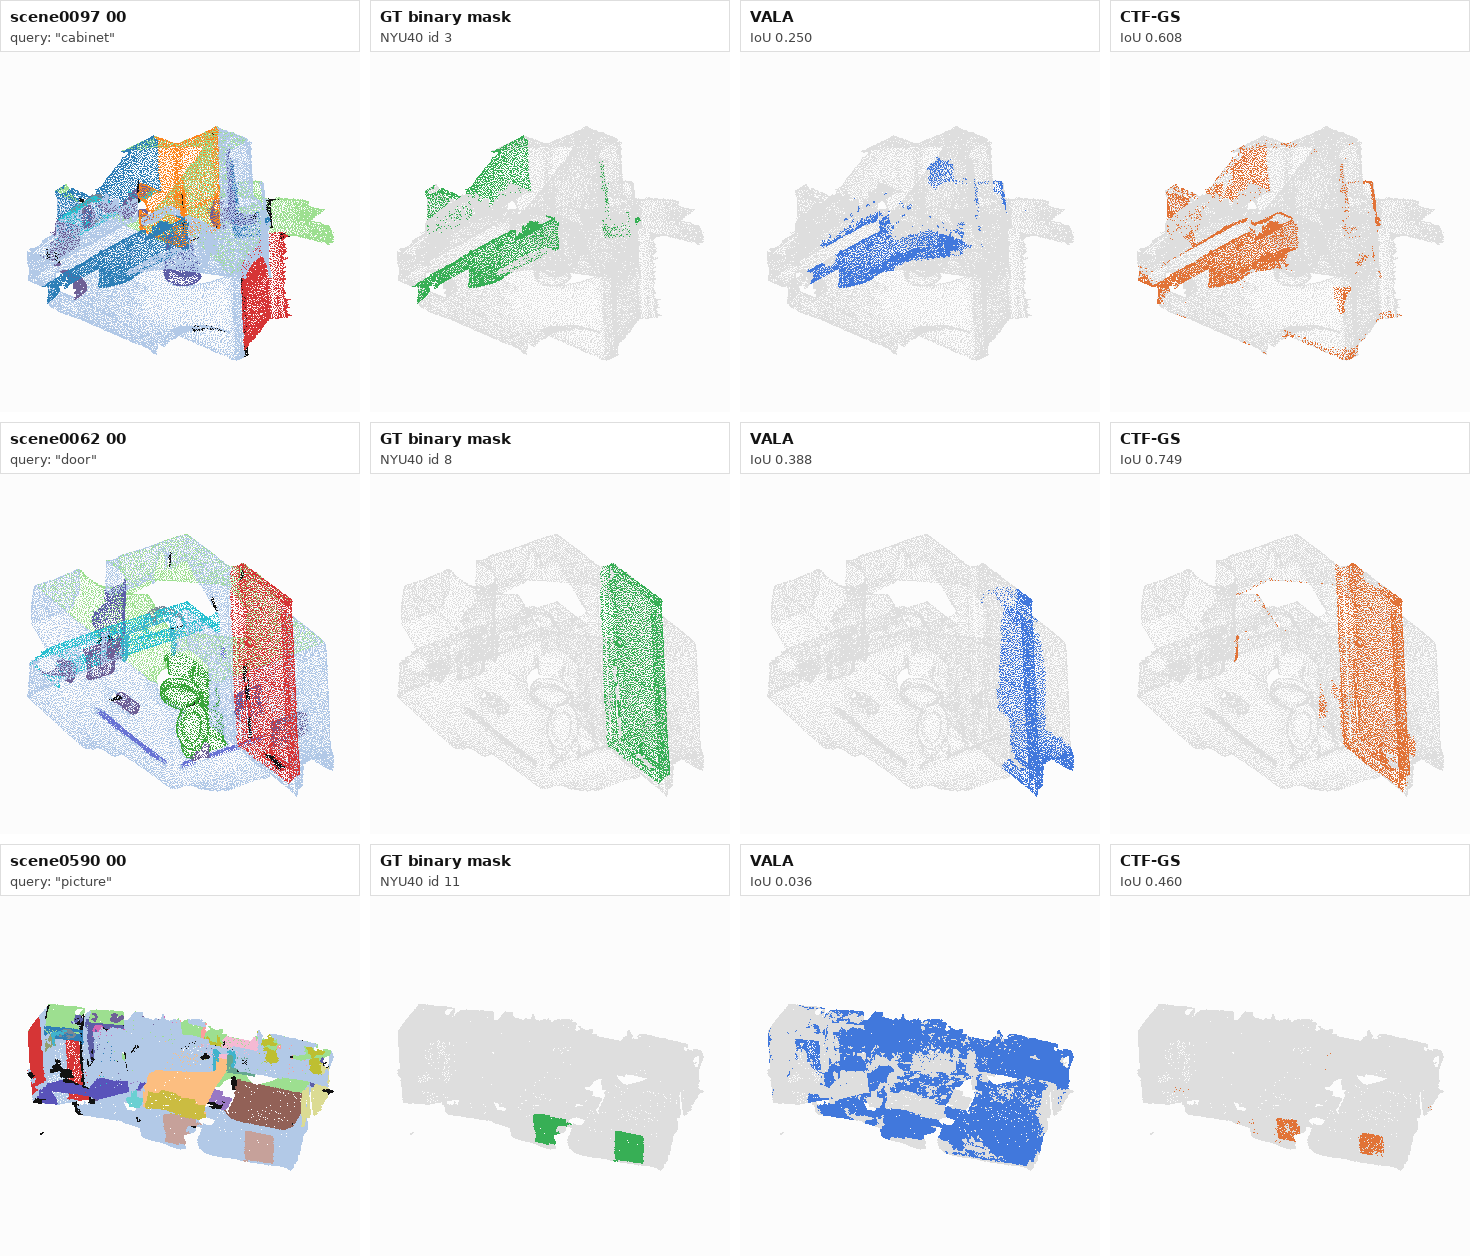
\includegraphics[width=\linewidth]{figures/scannet_openvocab_3d_query_qualitative.png}
\caption{ScanNet open-vocabulary 3D query qualitative comparison. Each row
shows a binary text-class query on a VALA-aligned ScanNet scene: scene overview, GT
class points, our local VALA compatibility reproduction, and \method{} direct
point-query prediction. Gray points are non-query classes.}
\label{fig:scannet_qualitative}
\end{figure*}

Fig.~\ref{fig:direct3d_ablation_qualitative} visualizes the direct-3D support-calibration
ablation on small or fragmented LERF queries. The base compact selector
uses primitive scores from the compact field, while the final selector adds the
prompt ensemble and label-free component-support calibration used by the deployed
compact direct query.

\begin{figure*}[t]
\centering
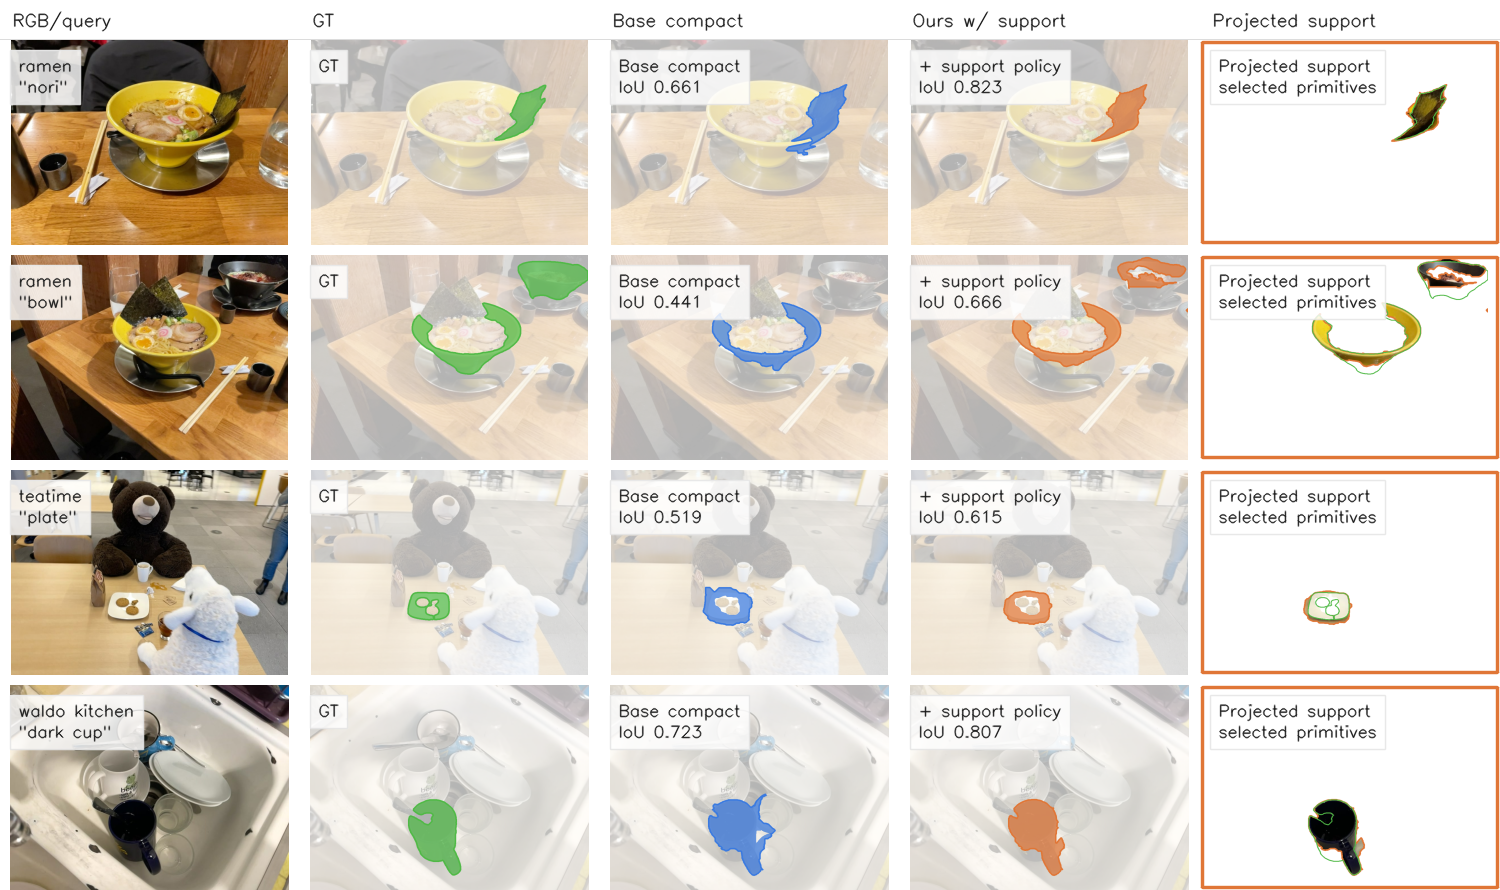
\includegraphics[width=\linewidth]{figures/lerf_direct3d_support_policy_ablation_qualitative.png}
\caption{Qualitative ablation of compact direct-3D support calibration. The
selector recovers small or fragmented object support without a multiview-registration feature
cache or official RGB SAM3 mask decoder; rendering is used only to visualize and
evaluate the selected 3D primitives.}
\label{fig:direct3d_ablation_qualitative}
\end{figure*}

Fig.~\ref{fig:rendered_boundary_qualitative} isolates the rendered-view
boundary calibration used by the feature-only SAM3-adaptor mask head. Unlike the
frozen official SAM3 diagnostic, this head is conditioned on reconstructed
CTF-GS/RADIO features and prompt embeddings; it does not call the official RGB
SAM3 decoder at evaluation time.

\begin{figure*}[t]
\centering
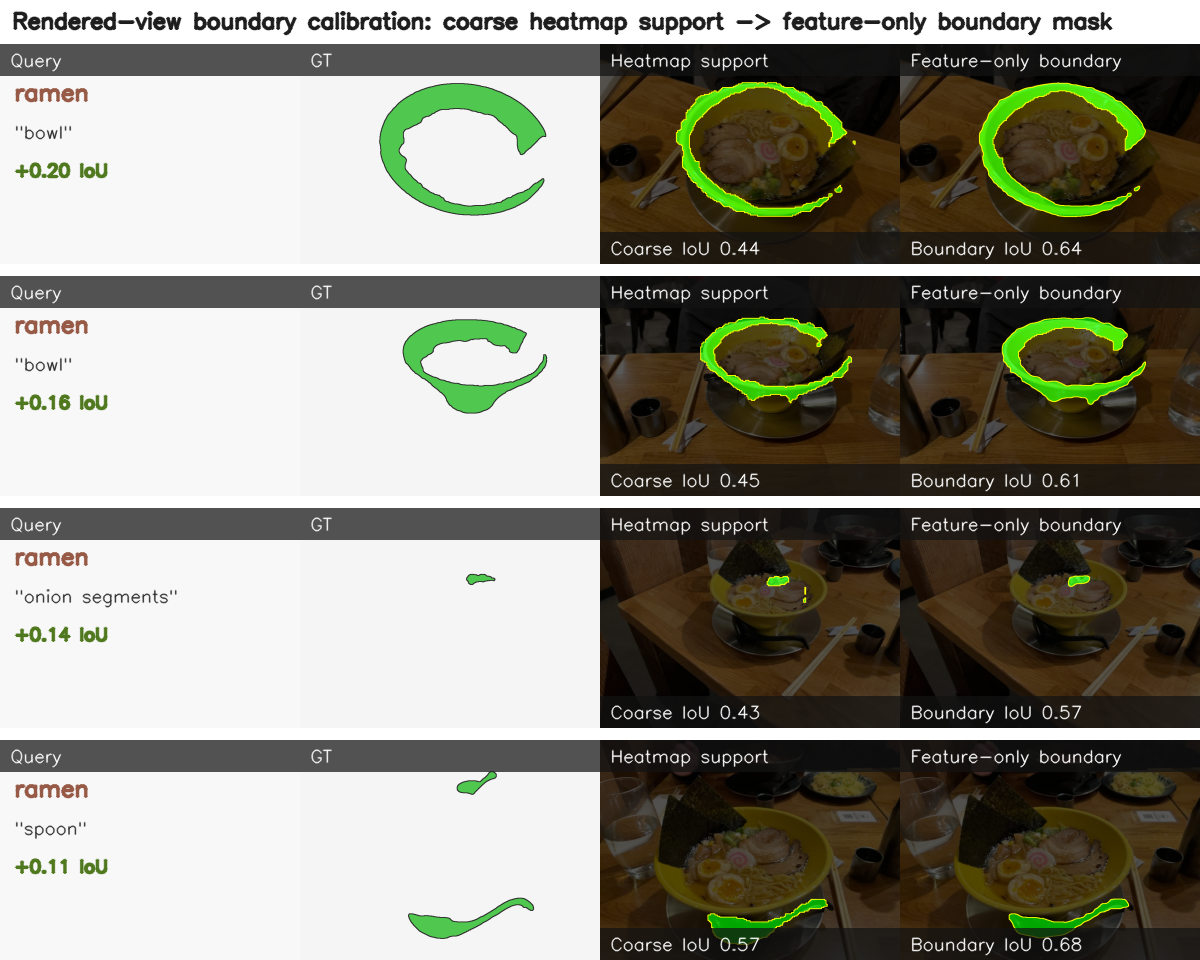
\includegraphics[width=\linewidth]{figures/lerf_rendered_boundary_calibration_qualitative.png}
\caption{Rendered-view boundary calibration qualitative examples. The coarse
heatmap support is converted into a feature-only boundary mask using the
prompt-conditioned SAM3-adaptor head. The examples show per-query IoU gains
without invoking an external RGB SAM3 decoder.}
\label{fig:rendered_boundary_qualitative}
\end{figure*}

Fig.~\ref{fig:teacher_field_qualitative} compares reconstructed scene features
with frame-wise RADIO features under the frozen downstream probes used in
Table~\ref{tab:sam_dino_tasks}. These examples visualize the same claim as the
quantitative probe table: the compact scene field is not merely a compressed
copy of a single view, but a multiview feature memory that can produce more
stable downstream responses.

\begin{figure*}[t]
\centering
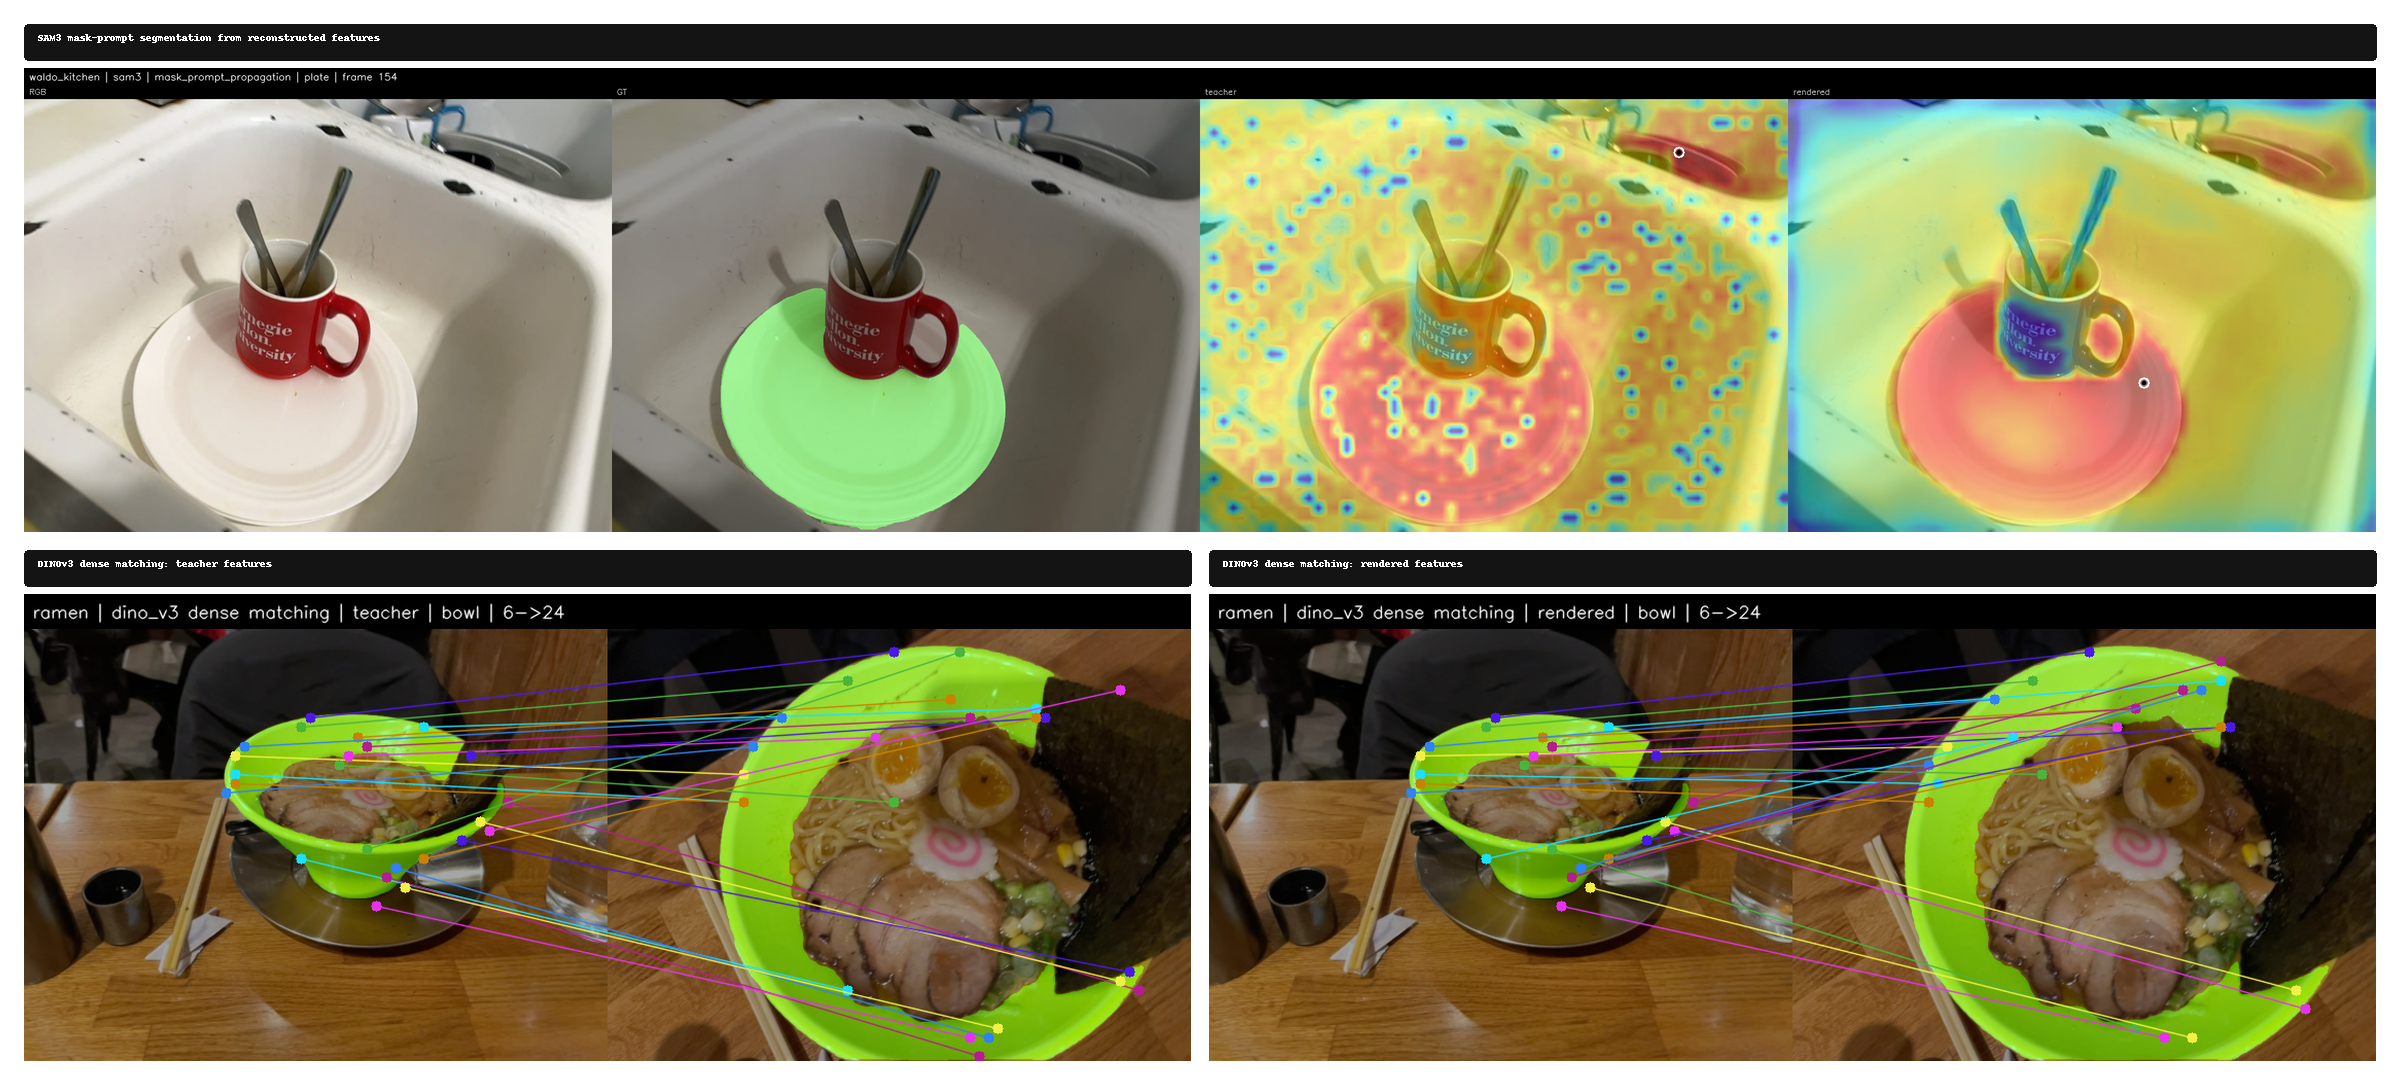
\includegraphics[width=\linewidth]{figures/lerf_sam_dino_tasks_qualitative.png}
\caption{Reconstructed scene features versus frame-wise RADIO under frozen-head
tasks. Columns compare the task input/GT, frame-wise RADIO response, and
\method{} reconstructed field response for SigLIP2 grounding, SAM3-adaptor mask
propagation, DINOv3 mask propagation, and DINOv3 dense matching.}
\label{fig:teacher_field_qualitative}
\end{figure*}

Additional rendered heatmap examples, alpha/depth boundary cases, and extended
SAM/DINO-adaptor controls are kept in the supplementary material so the main
paper focuses on one representative figure per claim.

\subsection{Failure Analysis}

\begin{table}[t]
\centering
\caption{Representative fragile LERF-OVS categories from the frozen rendered-feature evaluation. Low LocAcc with nonzero mIoU highlights the peak-vs-region trade-off.}
\label{tab:failure_analysis}
\begin{tabular}{llrr}
\toprule
Scene & Category & LocAcc & mIoU \\
\midrule
Figurines & bag & 0.00 & 0.00 \\
Figurines & miffy & 0.00 & 0.01 \\
Teatime & dall-e brand & 0.00 & 0.01 \\
Figurines & jake & 0.00 & 0.02 \\
Waldo Kitchen & ketchup & 0.00 & 0.03 \\
Waldo Kitchen & spatula & 0.00 & 0.03 \\
Ramen & corn & 0.00 & 0.10 \\
Figurines & red toy chair & 0.00 & 0.13 \\
\bottomrule
\end{tabular}
\end{table}


Table~\ref{tab:failure_analysis} turns the qualitative small-object observation
into a quantitative failure analysis. The lowest-ranked categories are mostly tiny or
visually ambiguous objects, such as Figurines bags, character toys, and isolated
kitchen tools. The failure pattern is not only low region overlap: some
categories show nonzero mIoU but zero or partial LocAcc, which means the
rendered heatmap covers a plausible object region while the single maximum lands
outside the annotated polygon. This is why the paper treats mIoU improvements
from adaptor or cross-view losses conservatively unless localization accuracy is
preserved.

\section{Discussion}

\paragraph{Why feature reconstruction matters.}
The LERF-OVS results show that rendered RADIO-like features retain enough
semantic structure for open-vocabulary localization. The ScanNet results suggest
that the same representation can be probed outside the LERF object-query setting.
The LERF direct-selection experiment further clarifies the boundary of this
claim: the compact field supports direct primitive querying, Multiview Primitive Registration provides an
auditable training bridge for primitive evidence, and support-calibrated
selection is needed to convert primitive scores into stable object masks. Bare
score-threshold selection is still weaker than object-aware grouping on
fragmented scenes, so we distinguish primitive scoring quality from boundary and
support calibration quality.

\paragraph{Baseline scope.}
The main LERF and ScanNet quantitative tables use the reproduced protocols
reported in this paper. Historical cross-paper provenance tables are retained
only as auxiliary audit material and are not the basis for the main ranking
claims.

\paragraph{Why the compact field can outperform frame-wise RADIO.}
\method{} is trained from frame-wise RADIO features, but its rendered query path is
not restricted to a single frame. Multiview reconstruction, visibility-aware
regularization, and support-calibrated selection can suppress view-specific noise and
recover a scene-consistent response. This explains why the rendered field can
outperform frame-wise RADIO under the same frozen SigLIP2, SAM3-adaptor, and
DINOv3 probe tasks, while still being limited by frame-wise feature resolution and
annotation ambiguity on small objects.

\section{Limitations}

\method{} depends on a pretrained Gaussian geometry backbone and does not claim
to improve RGB reconstruction. Small objects remain challenging because RADIO
feature resolution, Gaussian support density, and rendered feature alignment
limit heatmap sharpness. The ScanNet protocol is a direct point-query feature
probe, not a replacement for a full standardized semantic segmentation
benchmark. The main LERF and ScanNet tables use the reproduced protocols
reported in this paper; historical cross-paper provenance notes are kept only
for auditability. The deployed compact direct-3D result uses GT-free color-edge
and score-component support calibration. This does not invoke a learned RGB
segmentation network or official RGB SAM decoder, but it should be understood as
a lightweight support-calibration step rather than a completely image-free
selector. The frozen official SAM3 box result is therefore kept as a
post-selection diagnostic rather than the core compact-memory claim. The storage
table reports feature footprint separately from full checkpoint footprint; a
deployment package should keep the same separation between persistent feature
parameters, transient rendering buffers, and optional downstream heads.

\section{Conclusion}

\method{} turns a 3D Gaussian scene into a reusable compact foundation-feature
memory. Its central claim is deliberately narrower than generic semantic
Gaussian learning: a low-dimensional contextual Gaussian field can reconstruct
RADIO-compatible scene features, absorb sparse multiview primitive evidence, and
support rendered-view, direct-primitive, and point-level open-vocabulary
queries without deploying a high-dimensional multiview feature cache. The
LERF-OVS, direct-3D, ScanNet, frame-wise RADIO comparison, storage, latency, and
ablation results jointly support this claim. The remaining limitations are also
clear: small fragmented objects and boundary-sensitive queries still depend on
support calibration, and the ScanNet protocol should be interpreted as direct
foundation-feature probing rather than full semantic-segmentation replacement.
These boundaries make the result reproducible and falsifiable while preserving
the main contribution: compact reconstructive foundation features can be made a
first-class 3D scene representation.

\bibliographystyle{IEEEtran}
\bibliography{radio_gs_refs}

\end{document}
